% \section{Appendix: Deidentify.org}


\section{Chapter Summary}

This chapter demonstrated that de-identification of player tracking data is non-trivial to perform correctly, and that common de-identification approaches can lead to individual players being re-identified. Through comparing the trade-off between participant privacy and data quality, a combination of downsampling and representation as a point cloud were found to offer the best theoretical protection of individual privacy while still allowing team-based analysis.

\subsection*{Limitations}

% - 1 Hz not applicable to all sports
% - not suited to individual Analysis
% - not suited to situations where sport consists of player roles (or if players are not sufficiently mobile)
% 
% - Need to trust script
% - radically different approach may be needed outside of AFL

The de-identification approach has been selected for \afl{} where players can move freely on the field, but may not work well for other types of sport where players have set roles. Specifically, the de-identification scheme relies on players crossing paths in order to make it harder for an attacker to re-identify players; however, if a player maintains the same position (e.g. a cricket player that always fields in the same position) or rarely comes into close contact with other players, then the attacker could use this information to re-identify the player. Furthermore, by design, the de-identification only allows team-level analysis rather than individual player analysis. This means that the proposed approach is not appropriate for traditional forms of sport performance analysis that focus on analysing individual players, or specific player roles (e.g. in netball). An alternative de-identification approach would be needed for these forms of sport analysis. Nevertheless, the interaction model proposed is sufficiently general that the overall framework is still appropriate to these scenarios if a suitable de-identification operation can be found (e.g. the interaction model could be used to request summary data broken down by player role, but aggregated over multiple seasons in order to prevent re-identification risk).

\subsection*{Applied Output}

\begin{figure}[htp]
  \centering
  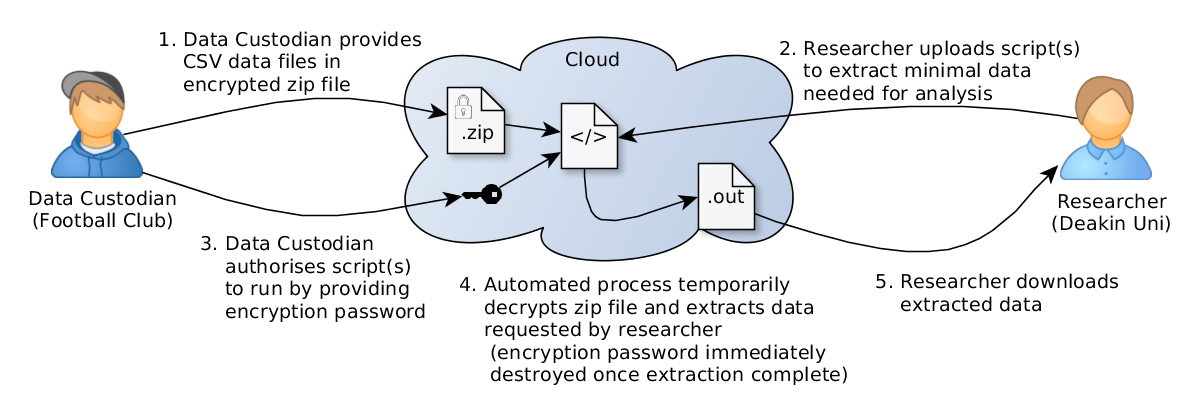
\includegraphics[width=\linewidth]{deidentify-portal/deidentification-pipeline.png}
  \caption{Summary of interaction model as implemented in \textit{deidentify.org} portal}
  \label{fig:deident-pipeline-summary}
\end{figure}

\begin{figure}[htp]
  \centering
  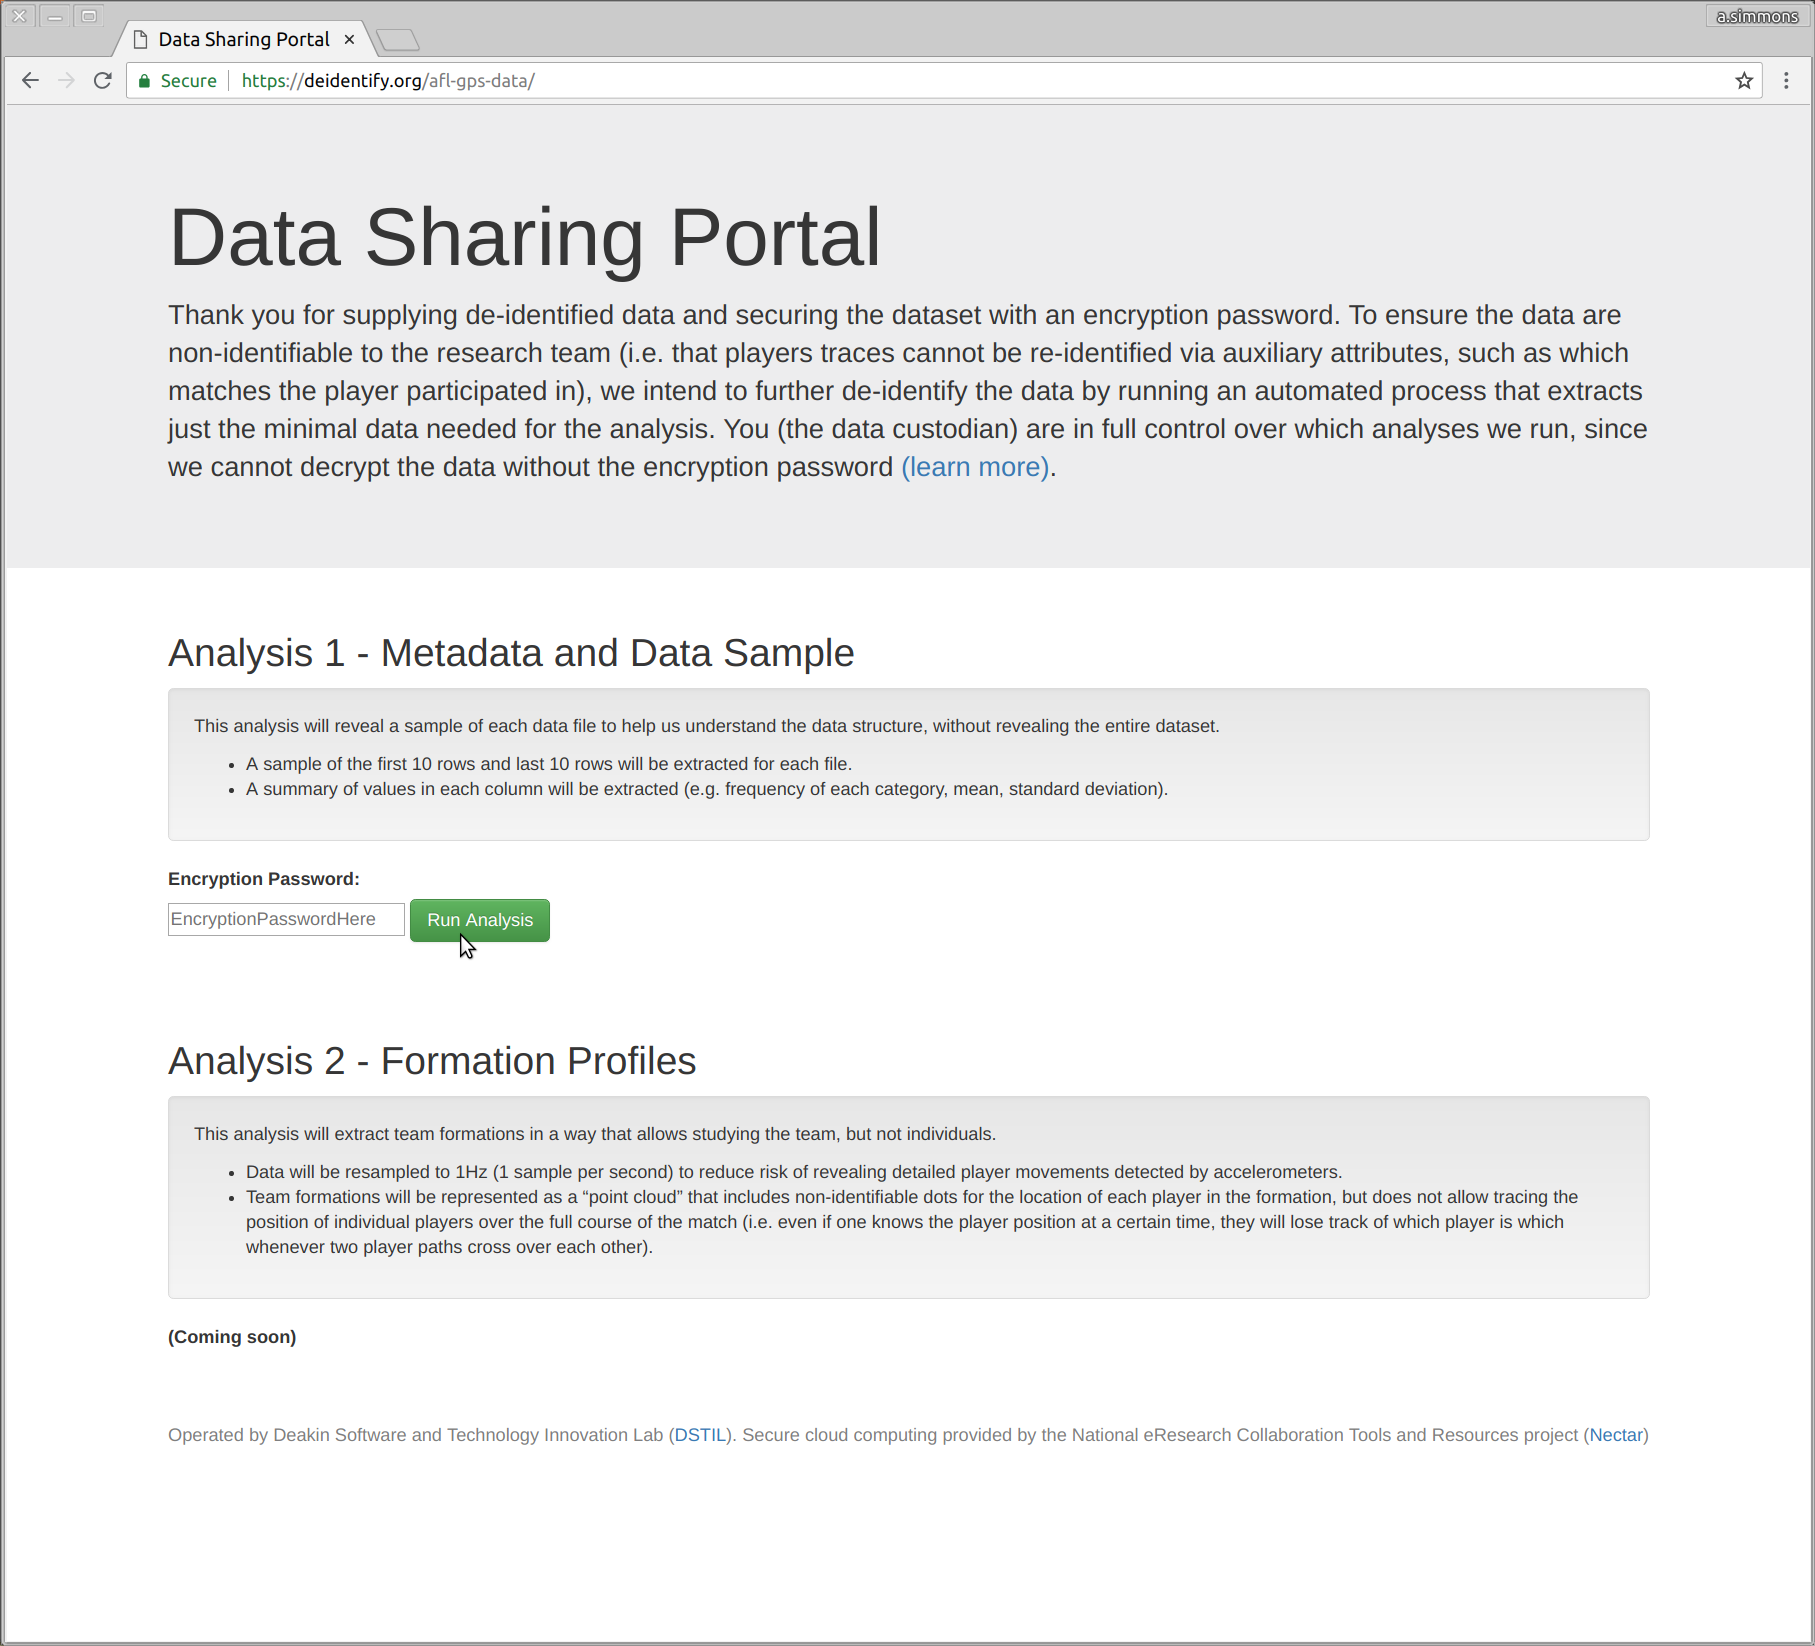
\includegraphics[width=\linewidth]{deidentify-portal/deidentification-portal-screenshot.png}
  \caption{Screenshot of \textit{deidentify.org} portal in use}
  \label{fig:deident-portal-screenshot}
\end{figure}

The research in this chapter was applied to develop the proof of concept de-identification portal \textit{deidentify.org}. This is a cloud service for data custodians to share data with researchers in a way that meets Victorian privacy legislation and Australian human research ethics guidelines for non-identifiable data. Unlike existing methods in which the data custodian substitutes names with anonymous identifiers then hands over the full `de-identified' dataset to researchers---which may still lead to re-identification or permit unethical uses if the dataset contains quasi-identifiers such as times, dates, or locations---\textit{deidentify.org} encourages researchers to write analysis programs that extract just the data they need, and gives the data custodian control over which analyses can run.

A summary of the interaction model for \textit{deidentify.org} is shown in \figref{fig:deident-pipeline-summary}, which can be seen to follow that of \secref{sec:deidentify-interactionmodel}. The \textit{deidentify.org} portal was used request the de-identified sport player tracking data used in this thesis. A screenshot of \textit{deidentify.org} in use is provided in \figref{fig:deident-portal-screenshot}.

\subsection*{Future Work}

A more robust implementation of the de-identification interaction model is needed before offering the system for general use and high risk research. This would require additional software engineering effort to allow the system to scale and auditing of the source code by a professional security analyst. In particular, if providing a public server for de-identification, there is a need to ensure that processes are correctly isolated to protect the data during the short time frame in which the raw data is decrypted on the server while the de-identification algorithm runs. An alternative would be to use \textit{homomorphic encryption}\footnote{For a high-level summary of the promises and practical limitations of homomorphic encryption see Andy Greenberg, 3 Nov 2014, ``Hacker Lexicon: What Is Homomorphic Encryption?'', Wired. \url{https://www.wired.com/2014/11/hacker-lexicon-homomorphic-encryption/}} to avoid the need to ever decrypt the data on the sever; however, the overhead of fully homomorphic encryption is currently impractical for computationally intensive operations on large datasets.

Additional work is also needed to test the usability of the system. The proposed system provides the data custodian the power to decide which analyses the researcher runs. However, currently, this requires a certain level of trust in the researcher to correctly state what each of their analysis scripts will extract. One option would be for the system to show the data custodian the source code of the analysis script that will be run as part of the approval process; however, as the system is designed to empower data custodians without programming expertise to safely share data, this is unlikely to provide any meaningful security if the data custodian does not understand the researcher's code. Thus a mechanism is needed to automatically audit the analysis script to confirm that it conforms to the human readable summary of what it will extract and to automatically test whether the analysis output leaks potentially sensitive information (e.g. by automatically running a series of re-identification attacks to test for common de-identification mistakes).

% - Need to study the number of interactions between players to confirm
% - Need to study on larger number of cases / with sport scientists
% - Need to study whether data custodians can determine whether or not to grant request
% - Consider standardising as part of ethics process

\subsection*{Contributions}

\begin{enumerate}
  \item Exposed the prevalence of improper de-identification methods used in sport research, and demonstrated that GPS player tracking data is particularly prone to re-identification. An interaction model was proposed to help improve ethical conduct of research by allowing the researcher to specify the de-identification operations in cases where the data custodian lacks the technical resources to strongly de-identify data themselves prior to data hand-over. The proposed approach was applied to GPS player tracking data held by an AFL club to obtain the non-identifiable data used in this thesis.
\end{enumerate}
